%-----------------------------------LICENSE------------------------------------%
%   This file is part of Mathematics-and-Physics.                              %
%                                                                              %
%   Mathematics-and-Physics is free software: you can redistribute it and/or   %
%   modify it it under the terms of the GNU General Public License as          %
%   published by the Free Software Foundation, either version 3 of the         %
%   License, or (at your option) any later version.                            %
%                                                                              %
%   Mathematics-and-Physics is distributed in the hope that it will be useful, %
%   but WITHOUT ANY WARRANTY; without even the implied warranty of             %
%   MERCHANTABILITY or FITNESS FOR A PARTICULAR PURPOSE.  See the              %
%   GNU General Public License for more details.                               %
%                                                                              %
%   You should have received a copy of the GNU General Public License along    %
%   with Mathematics-and-Physics.  If not, see <https://www.gnu.org/licenses/>.%
%------------------------------------------------------------------------------%

%   Use the standalone class for displaying the tikz image on a small PDF.
\documentclass[crop, tikz]{standalone}

%   Import the tikz package to use for the drawing.
\usepackage{tikz}

%   The arrows package is used for the LaTeX arrow.
\usetikzlibrary{arrows.meta}

%   Begin the document.
\begin{document}

    %   Begin the drawing.
    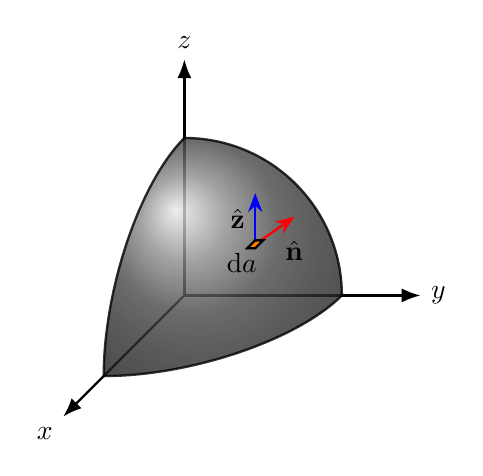
\begin{tikzpicture}[%
        line width=0.3mm,%
        line cap=round,%
        >={Latex},%
        every edge/.style={%
            draw=black,%
            very thick%
        }%
    ]

        %   Draw the coordinate axes.
        \draw[->] (0.0, 0.0, 0.0) -- (3.0, 0.0, 0.0) node[right] {$y$};
        \draw[->] (0.0, 0.0, 0.0) -- (0.0, 3.0, 0.0) node[above] {$z$};
        \draw[->] (0.0, 0.0, 0.0) -- (0.0, 0.0, 4.0) node[below left] {$x$};

        %   Color in the sphere.
        \draw[ball color=black!60!white,opacity=0.8]
            (2.0, 0.0) arc (0:90:2)
            {[x={(0.0, 0.0, 1.33)}] arc (90:0:2)}
            {[y={(0.0, 0.0, 1.33)}] arc (90:0:2)};

        %   Draw an arrow for the z direction.
        \draw[->, >=Stealth, draw=blue]
            (0.9, 0.65) -- node [left] {$\hat{\mathbf{z}}$} (0.9, 1.3);

        %   And an arrow for the normal.
        \draw[->, >=Stealth, draw=red]
            (0.9, 0.65) -- node [below right] {$\hat{\mathbf{n}}$} (1.4, 1.0);

        %   Fill in the tiny area on the sphere.
        \draw[fill=orange]
            (0.8, 0.6) to (0.9, 0.6) to (1, 0.7) to (0.9, 0.7) to cycle;

        %   Label the infinitesimal area.
        \node at (0.73, 0.67) [below] {$\textrm{d}a$};
    \end{tikzpicture}
\end{document}
